\documentclass[preprint, 3p,
authoryear]{elsarticle} %review=doublespace preprint=single 5p=2 column
%%% Begin My package additions %%%%%%%%%%%%%%%%%%%

\usepackage[hyphens]{url}

  \journal{Biogeochemistry} % Sets Journal name

\usepackage{lineno} % add
  \linenumbers % turns line numbering on

\usepackage{graphicx}
%%%%%%%%%%%%%%%% end my additions to header

\usepackage[T1]{fontenc}
\usepackage{lmodern}
\usepackage{amssymb,amsmath}
\usepackage{ifxetex,ifluatex}
\usepackage{fixltx2e} % provides \textsubscript
% use upquote if available, for straight quotes in verbatim environments
\IfFileExists{upquote.sty}{\usepackage{upquote}}{}
\ifnum 0\ifxetex 1\fi\ifluatex 1\fi=0 % if pdftex
  \usepackage[utf8]{inputenc}
\else % if luatex or xelatex
  \usepackage{fontspec}
  \ifxetex
    \usepackage{xltxtra,xunicode}
  \fi
  \defaultfontfeatures{Mapping=tex-text,Scale=MatchLowercase}
  \newcommand{\euro}{€}
\fi
% use microtype if available
\IfFileExists{microtype.sty}{\usepackage{microtype}}{}
\usepackage[]{natbib}
\bibliographystyle{plainnat}

\usepackage{graphicx}
\ifxetex
  \usepackage[setpagesize=false, % page size defined by xetex
              unicode=false, % unicode breaks when used with xetex
              xetex]{hyperref}
\else
  \usepackage[unicode=true]{hyperref}
\fi
\hypersetup{breaklinks=true,
            bookmarks=true,
            pdfauthor={},
            pdftitle={How is Mercury Correlated with Dissolved Organic Carbon in Streams?},
            colorlinks=false,
            urlcolor=blue,
            linkcolor=magenta,
            pdfborder={0 0 0}}

\setcounter{secnumdepth}{5}
% Pandoc toggle for numbering sections (defaults to be off)

% Pandoc syntax highlighting
\usepackage{color}
\usepackage{fancyvrb}
\newcommand{\VerbBar}{|}
\newcommand{\VERB}{\Verb[commandchars=\\\{\}]}
\DefineVerbatimEnvironment{Highlighting}{Verbatim}{commandchars=\\\{\}}
% Add ',fontsize=\small' for more characters per line
\usepackage{framed}
\definecolor{shadecolor}{RGB}{248,248,248}
\newenvironment{Shaded}{\begin{snugshade}}{\end{snugshade}}
\newcommand{\AlertTok}[1]{\textcolor[rgb]{0.94,0.16,0.16}{#1}}
\newcommand{\AnnotationTok}[1]{\textcolor[rgb]{0.56,0.35,0.01}{\textbf{\textit{#1}}}}
\newcommand{\AttributeTok}[1]{\textcolor[rgb]{0.77,0.63,0.00}{#1}}
\newcommand{\BaseNTok}[1]{\textcolor[rgb]{0.00,0.00,0.81}{#1}}
\newcommand{\BuiltInTok}[1]{#1}
\newcommand{\CharTok}[1]{\textcolor[rgb]{0.31,0.60,0.02}{#1}}
\newcommand{\CommentTok}[1]{\textcolor[rgb]{0.56,0.35,0.01}{\textit{#1}}}
\newcommand{\CommentVarTok}[1]{\textcolor[rgb]{0.56,0.35,0.01}{\textbf{\textit{#1}}}}
\newcommand{\ConstantTok}[1]{\textcolor[rgb]{0.00,0.00,0.00}{#1}}
\newcommand{\ControlFlowTok}[1]{\textcolor[rgb]{0.13,0.29,0.53}{\textbf{#1}}}
\newcommand{\DataTypeTok}[1]{\textcolor[rgb]{0.13,0.29,0.53}{#1}}
\newcommand{\DecValTok}[1]{\textcolor[rgb]{0.00,0.00,0.81}{#1}}
\newcommand{\DocumentationTok}[1]{\textcolor[rgb]{0.56,0.35,0.01}{\textbf{\textit{#1}}}}
\newcommand{\ErrorTok}[1]{\textcolor[rgb]{0.64,0.00,0.00}{\textbf{#1}}}
\newcommand{\ExtensionTok}[1]{#1}
\newcommand{\FloatTok}[1]{\textcolor[rgb]{0.00,0.00,0.81}{#1}}
\newcommand{\FunctionTok}[1]{\textcolor[rgb]{0.00,0.00,0.00}{#1}}
\newcommand{\ImportTok}[1]{#1}
\newcommand{\InformationTok}[1]{\textcolor[rgb]{0.56,0.35,0.01}{\textbf{\textit{#1}}}}
\newcommand{\KeywordTok}[1]{\textcolor[rgb]{0.13,0.29,0.53}{\textbf{#1}}}
\newcommand{\NormalTok}[1]{#1}
\newcommand{\OperatorTok}[1]{\textcolor[rgb]{0.81,0.36,0.00}{\textbf{#1}}}
\newcommand{\OtherTok}[1]{\textcolor[rgb]{0.56,0.35,0.01}{#1}}
\newcommand{\PreprocessorTok}[1]{\textcolor[rgb]{0.56,0.35,0.01}{\textit{#1}}}
\newcommand{\RegionMarkerTok}[1]{#1}
\newcommand{\SpecialCharTok}[1]{\textcolor[rgb]{0.00,0.00,0.00}{#1}}
\newcommand{\SpecialStringTok}[1]{\textcolor[rgb]{0.31,0.60,0.02}{#1}}
\newcommand{\StringTok}[1]{\textcolor[rgb]{0.31,0.60,0.02}{#1}}
\newcommand{\VariableTok}[1]{\textcolor[rgb]{0.00,0.00,0.00}{#1}}
\newcommand{\VerbatimStringTok}[1]{\textcolor[rgb]{0.31,0.60,0.02}{#1}}
\newcommand{\WarningTok}[1]{\textcolor[rgb]{0.56,0.35,0.01}{\textbf{\textit{#1}}}}

% tightlist command for lists without linebreak
\providecommand{\tightlist}{%
  \setlength{\itemsep}{0pt}\setlength{\parskip}{0pt}}



\usepackage{float}



\begin{document}


\begin{frontmatter}

  \title{How is Mercury Correlated with Dissolved Organic Carbon in
Streams?}
    \author[University of Regina]{Faraz Khan%
  \corref{cor1}%
  \fnref{1}}
   \ead{farazkhan@uregina.ca} 
    \author[University of Regina]{Britt Hall%
  %
  \fnref{1}}
   \ead{britt.hall@uregina.ca} 
      \affiliation[Some Institute of Technology]{Department, Street,
City, State, Zip}
    \affiliation[Another University]{Department, Street, City, State,
Zip}
    \cortext[cor1]{Corresponding author}
  
  \begin{abstract}
  Levels of dissolved organic carbon and mercury in streams.
  \end{abstract}
    \begin{keyword}
    methylmercury \sep 
    dissolved organic carbon
  \end{keyword}
  
 \end{frontmatter}

\hypertarget{introduction}{%
\section{Introduction}\label{introduction}}

Dissolved organic carbon (DOC) is highly associated with methylmercury
production in freshwater ecosystems. The use of optical instruments such
as spectrometers in the study of DOC have led to a greater understanding
of the chemical characteristics and origin of DOC. State of the art
emission excitation matrices analysis have resulted in a greater
understanding of DOC and its associations with MeHg in various
freshwater systems such as streams. \citep{Graham2013}.

\hypertarget{methods}{%
\section{Methods}\label{methods}}

To test these hypotheses, I will sample urban artificial wetlands and
wet ponds from sites across Regina and Saskatoon, using methods derived
from Strickman and Mitchell (2017). I will then use sediment samples
from these sites in mercury methylation assays involving isotope
dilution-gas chromatography-inductively coupled plasma mass
spectrometry. Samples will be enriched with a stable Hg isotope to
determine the Hg methylation rate constants, ambient Hg, and MeHg
concentrations.

\hypertarget{results}{%
\section{Results}\label{results}}

Figure \ref{fig1} is generated using an R chunk.

\begin{Shaded}
\begin{Highlighting}[]
\FunctionTok{setwd}\NormalTok{(}\StringTok{"\textasciitilde{}/ldpminiproject/Data"}\NormalTok{)}

\NormalTok{mercurydata }\OtherTok{\textless{}{-}} \FunctionTok{read\_csv}\NormalTok{(}\StringTok{"mercurydata.csv"}\NormalTok{)}
\end{Highlighting}
\end{Shaded}

\begin{verbatim}
## Rows: 29 Columns: 5
## -- Column specification --------------------------------------------------------
## Delimiter: ","
## chr (2): collection_site, collection_month
## dbl (3): mean_doc, mean_streamwater_mehg, chironomid_mehg
## 
## i Use `spec()` to retrieve the full column specification for this data.
## i Specify the column types or set `show_col_types = FALSE` to quiet this message.
\end{verbatim}

\begin{Shaded}
\begin{Highlighting}[]
\NormalTok{mercurydata}
\end{Highlighting}
\end{Shaded}

\begin{verbatim}
## # A tibble: 29 x 5
##    collection_site collection_month mean_doc mean_streamwater_m~ chironomid_mehg
##    <chr>           <chr>               <dbl>               <dbl>           <dbl>
##  1 Bartlett Brook  May                  3.82                0.23           337. 
##  2 Bartlett Brook  June                 3.82                0.23           413. 
##  3 Bartlett Brook  July                 3.82                0.23           379. 
##  4 Beck Brook      May                  2.09                0.03            83.4
##  5 Beck Brook      June                 2.09                0.03            86.8
##  6 Beck Brook      July                 2.09                0.03           137. 
##  7 Blodgett North  May                  8.68                0.57           378. 
##  8 Blodgett North  June                 8.68                0.57           438. 
##  9 Blodgett North  July                 8.68                0.57           364. 
## 10 Blodgett South  May                  3.82                0.11           316. 
## # ... with 19 more rows
\end{verbatim}

\begin{Shaded}
\begin{Highlighting}[]
\FunctionTok{ggplot}\NormalTok{(}\AttributeTok{data =}\NormalTok{ mercurydata, }
       \AttributeTok{mapping =} \FunctionTok{aes}\NormalTok{(}\AttributeTok{x =}\NormalTok{ mean\_doc , }\AttributeTok{y =}\NormalTok{ mean\_streamwater\_mehg)) }\SpecialCharTok{+}
  \FunctionTok{geom\_point}\NormalTok{()}
\end{Highlighting}
\end{Shaded}

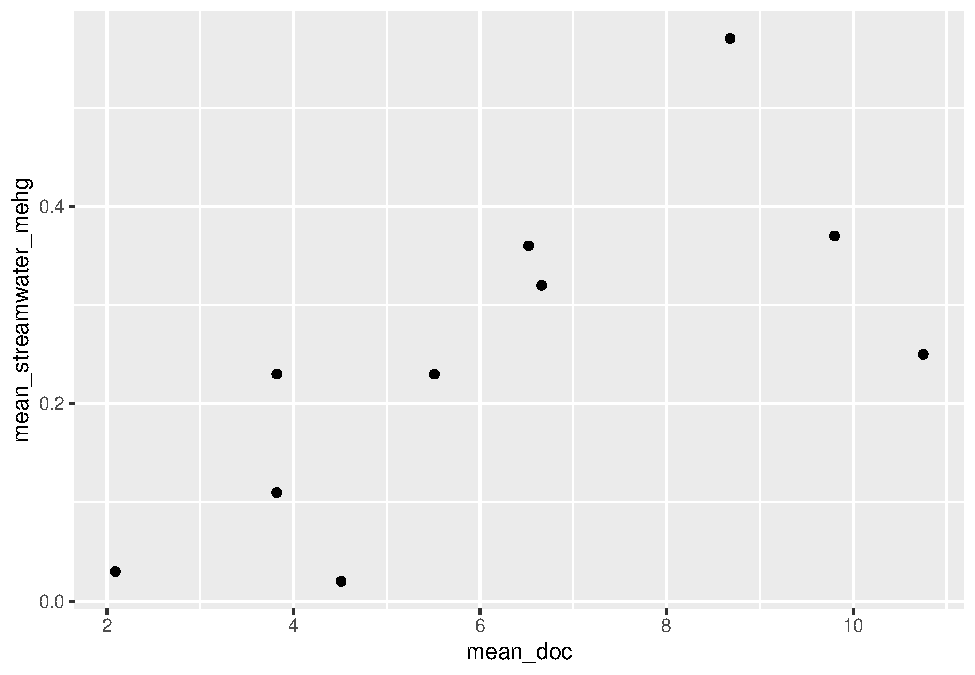
\includegraphics{ManususcriptRMarkdown_files/figure-latex/unnamed-chunk-1-1.pdf}

\begin{Shaded}
\begin{Highlighting}[]
\FunctionTok{setwd}\NormalTok{(}\StringTok{"\textasciitilde{}/ldpminiproject"}\NormalTok{)}
\end{Highlighting}
\end{Shaded}

\hypertarget{discussion}{%
\section{Discussion}\label{discussion}}

The results may be able to influence landscape planning and facilitate
further insight into the relationship between methylmercury and
bioavailability of inorganic mercury in urban environments. A great
understanding of the interactions in our built environment and how it
contributes to human caused ubiquitous ecological disruption (Policy
Horizons 2018) can ensure that we, as a society, move towards more
sustainable models of development. Benthic invertebrates are commonly
used as indicators of stream water quality \citep{Lescord2018}.
\emph{Baetis} sp. (Ephemeroptera) are used as stream quality indicators
for catchments \citep{Waiser2006}.

\renewcommand\refname{References}
\bibliography{mybibfile.bib}


\end{document}
